\chapter{Introducción}
\label{cap:introduccion}

\chapterquote{La inteligencia es la habilidad de adaptarse a los cambios}{Stephen Hawking}

\begin{resumen} En este capítulo se explicará la Motivación \ref{cap1:sec:Motivacion}, los objetivos que se quieren lograr inicialmente\ref{cap1:sec:Objetivos} y la estructura de esta memoria de TFG \ref{cap1:sec:Estructura}. 
\end{resumen}
\section{Motivación}
\label{cap1:sec:Motivacion}

Los humanos siempre hemos tenido la necesidad inherente de comunicarnos y quien no es capaz de hacerlo, generalmente acaba excluido. Y esa es la palabra clave, comunicación. Su origen proviene del latín, “\textit{communicare}”, difundir y este de “\textit{communis}” común. Gracias a ello, hemos podido llegar hasta donde estamos actualmente, una era donde todos pueden tener una voz. Por eso es más importante que nunca, no olvidarse de los que tienen dificultades. Para que puedan alzar su voz y difundir su palabra.

Sin embargo, en las últimas décadas ha habido un avance sin precedentes en el estudio e investigación sobre las discapacidades comunicativas. Éstos avances vinieron acompañados de herramientas y sistemas para facilitar la comunicación muchos de los cuales siguen vigentes a día de hoy. Uno de los principales perfiles que utilizan estos sistemas, son las  personas con trastorno del espectro autista (TEA)

Sin entrar en gran detalle, podemos encontrar que la gente con \textit{TEA} tienen dificultades en la comunicación verbal pues a menudo la comunicación no es recíproca o no se realiza en el contexto social adecuado. Respecto a la comunicación no verbal, también sufren dificultades al entender el significado de gestos faciales o expresión corporal de otras personas. Todo esto causa a menudo malentendidos, pues generalmente no se comprende el contexto y dificulta la comunicación. 

Para facilitar la comunicación se utilizan otros medios alternativos como los sistemas pictográficos, que permiten comunicarse mediante imágenes. Estos sitemas pictográficos, al estar compuestos por cientos de pictogramas habitualmente, están agrupados en \textbf{tableros pictográficos}. Estos tableros son superficies donde se colocan pictogramas para formar mensajes. Un ejemplo de tablero es el que vemos en la Figura \ref{fig:tablerofisico}. Hasta hace poco, dichos tableros eran creados a mano recortando y pegando los pictogramas pero con el tiempo se han desarrollado herramientas enfocadas a trabajar con tableros y pictogramas.

Para la elaboración de nuestra aplicación web tendremos en cuenta las aplicaciones de Pictar y PicTableros ya que ambos implementan herramientas que nos serán útiles de cara a la implementación. 

Durante este tiempo, además de estas herramientas, han surgido muchas más, cada una con sus características y funcionalidades únicas. Pero al final queda la sensación que nunca se podía hacer todo en un mismo lugar, y lo que le falta a una lo tiene otra herramienta, etc. Por ejemplo en las aplicaciones mencionadas previamente podemos ver que falta algún tipo de cuadrícula en el tablero para que a la hora de insertar los pictogramas estos queden perfectamente colocados y el tablero tenga una mejor apariencia visual.

En este contexto, la finalidad es crear una herramienta que unifique las mejores características de cada aplicación, además de permitir crear y editar tableros en un mismo lugar con la mayor facilidad posible. Afortunadamente, ya existe una base con la que nos podemos apoyar, gracias a proyectos de años anteriores como hemos mencionado, con ideas que se quedaron como trabajo futuro junto a las ideas propias. 


% TODO: \usepackage{graphicx} required
\begin{figure}[h!]
	\centering
	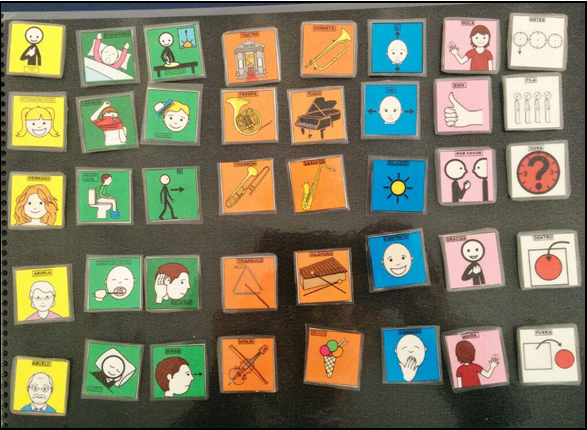
\includegraphics[width=0.7\linewidth]{Imagenes/Bitmap/tablerofisico}
	\caption{Tablero pictográfico en el que el usuario señala lo que quiere comunicar.}
	\label{fig:tablerofisico}
\end{figure}






\section{Objetivos}
\label{cap1:sec:Objetivos}

Teniendo en cuenta todos los temas que hemos tratado en la introducción queremos desarrollar una aplicación web multiplataforma que permite la edición de tableros y que incorpore una cuadrícula para ayudar a ajustar los pictogramas cuando se inserten. En la aplicación también se incorporarán herramientas de búsquedas de pictogramas por palabras y traducción de texto a pictograma.

Otro objetivo que nos hemos propuesto es que la aplicación pueda utilizarse en dos idiomas, por defecto la aplicación estará en español pero con una casilla para seleccionar el idioma se podrá cambiar a inglés. Este objetivo es sobre todo para ayudar y facilitar en el uso de esta aplicación a personas que no hablen español.

Para poder cumplir todos los objetivos mencionados se tendrá como referencia los TFG y TFM de Pictar y PicTableros. También se hará una labor de investigación en busca de nuevas tecnologías y herramientas con las que trabajar para desarrollar la aplicación. 

La forma en la que se comprobará el estado de los objetivos y su evolución será por medio de reuniones con los directores del TFG donde se analizará el trabajo realizado para ver el progreso, la forma en la que se van implementando los objetivos y la corrección de errores.



\section{Estructura de la memoria}
\label{cap1:sec:Estructura}

La estructura para memoria se encuentra dividida en [x] capítulos, a continuación se explicará brevemente su contenido. --según avancemos habrá que ir completándolo--
\begin{itemize}
	\item En los capítulos 1 y 2, se expondrá el contexto bajo el cual se ha realizado el trabajo junto a la motivación y objetivos para realizarlo.
	\item En el capítulo 3 se explicará qué es un pictograma y los distintos sistemas de comunicación con ellos. Además se analizarán las distintas herramientas relacionadas con pictogramas haciendo énfasis en la edición de tableros.
\end{itemize}	




